\documentclass[12pt]{article}
\usepackage{amsmath}
\usepackage{graphicx}
\usepackage{subcaption}
\setlength{\parindent}{0pt}
\setlength{\parskip}{10pt} % block paragraphs
\usepackage{bm}
\begin{document}

\title*{\centerline{\huge{CAP 5619 \-- Deep and Reinforcement Learning}}}
\author*{\centerline{HW3 Hua Huang}}%unnumbered centered head

\section {Problem 1}
(1) 
\begin{figure}[h]
    \centering
    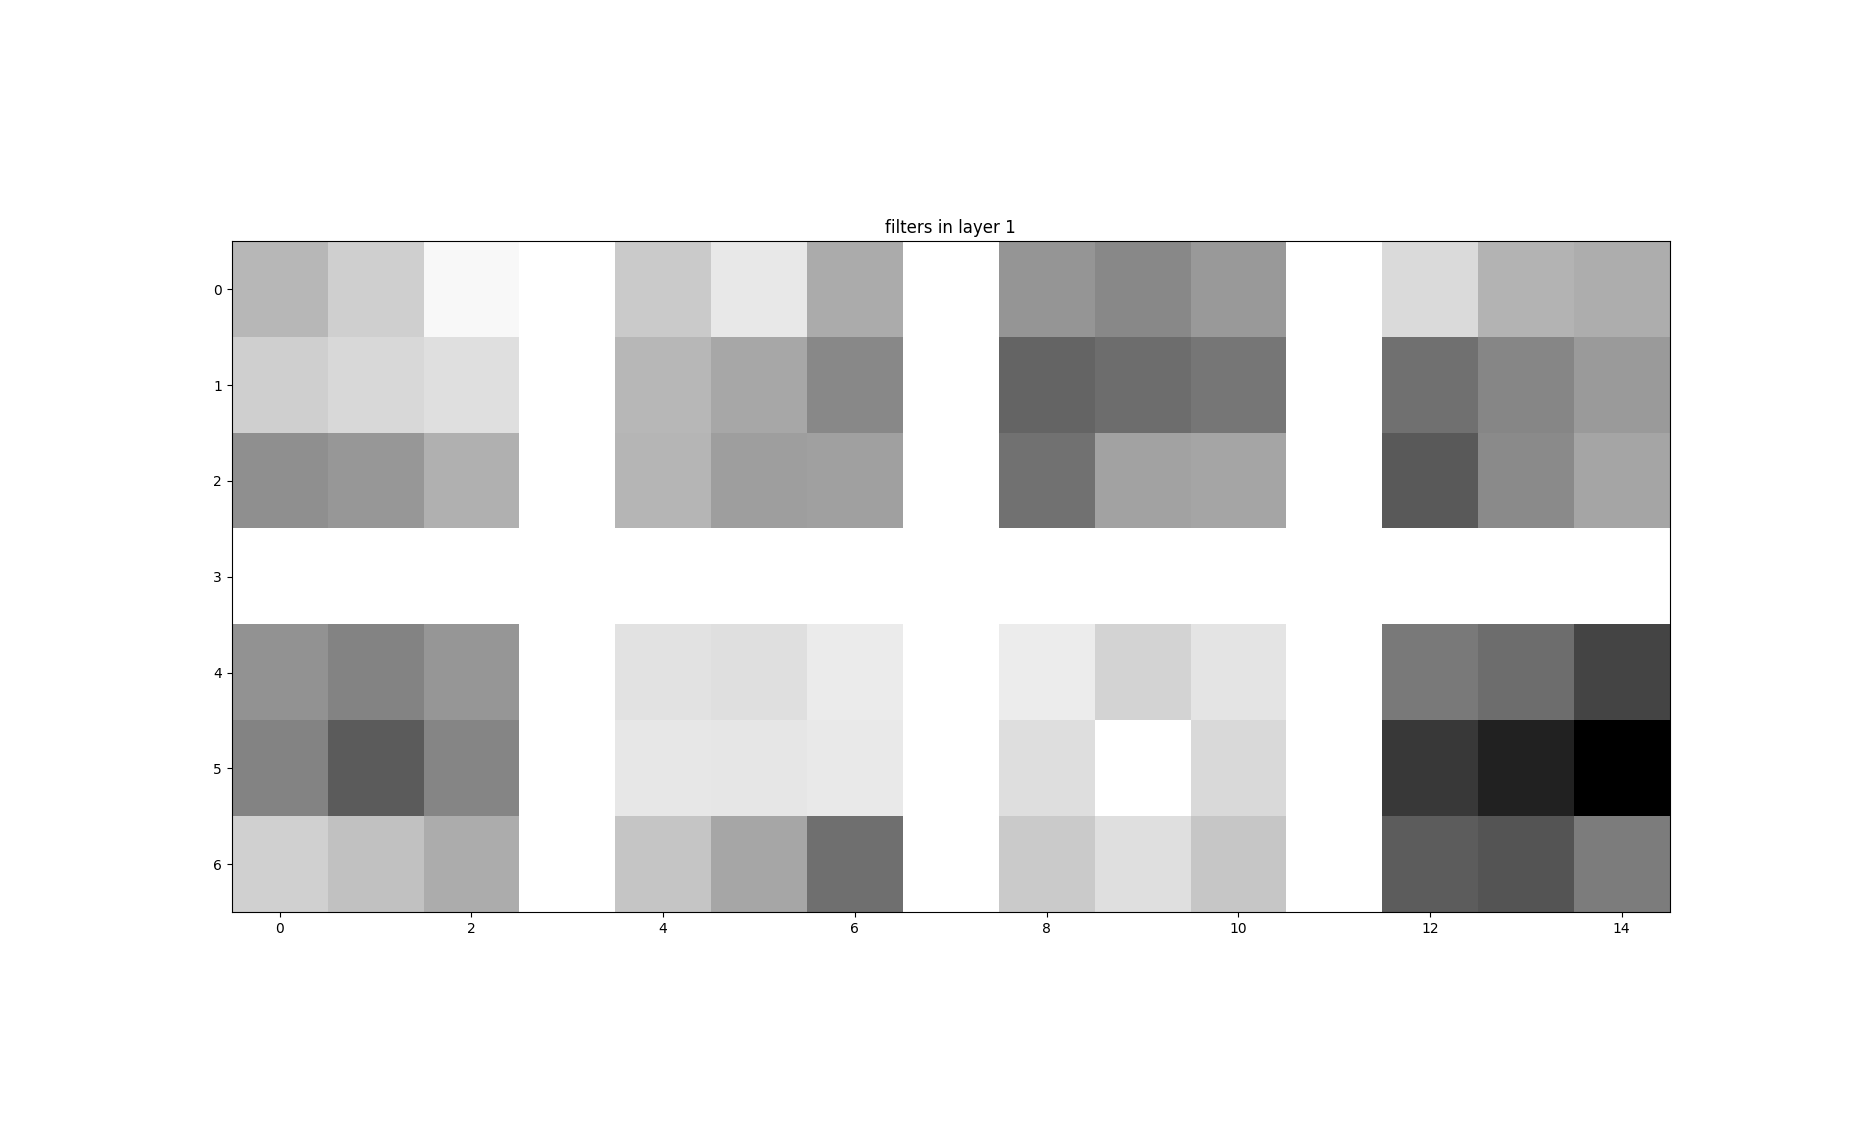
\includegraphics [scale=0.3]{filters_layer1.png}
    \caption {filters at layer 1}
\end{figure}

\begin{figure}[h]
    \centering
    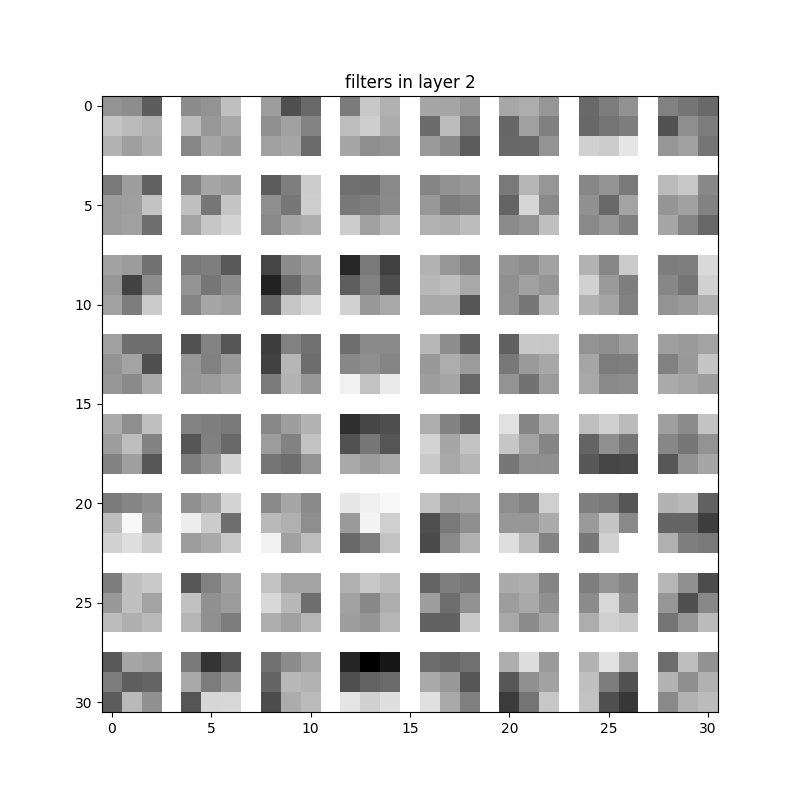
\includegraphics [scale=0.5]{filters_layer2.png}
    \caption {filters at layer 2}
\end{figure}

\begin{figure}[h]
    \centering
    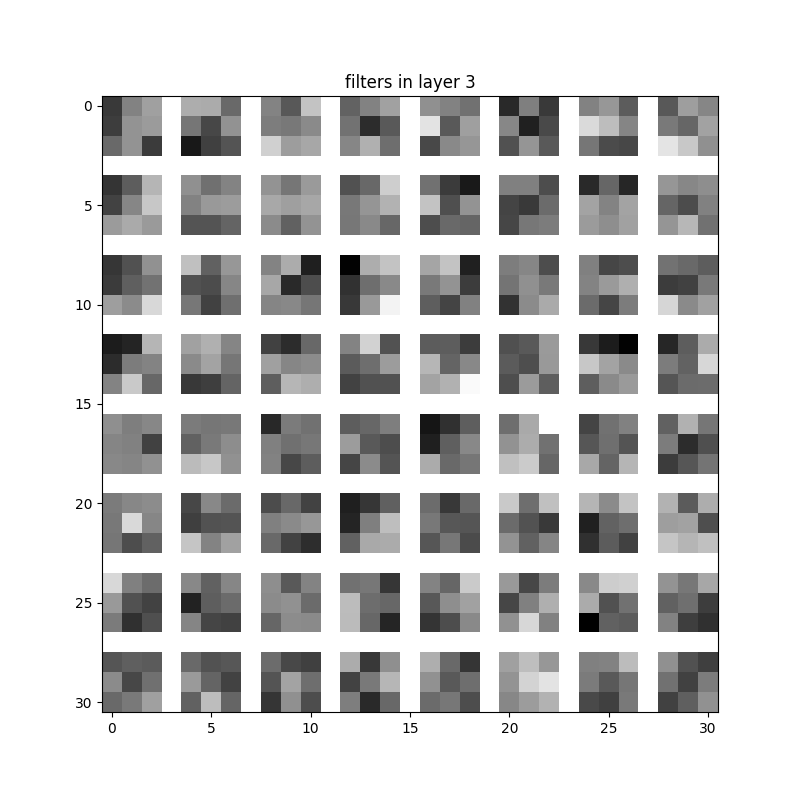
\includegraphics [scale=0.5]{filters_layer3.png}
    \caption {filters at layer 3}
\end{figure}
\clearpage

(2) Yes, we can still see clearly they are basically $0$ and $8$. 
\begin{figure}[h]
    \centering
    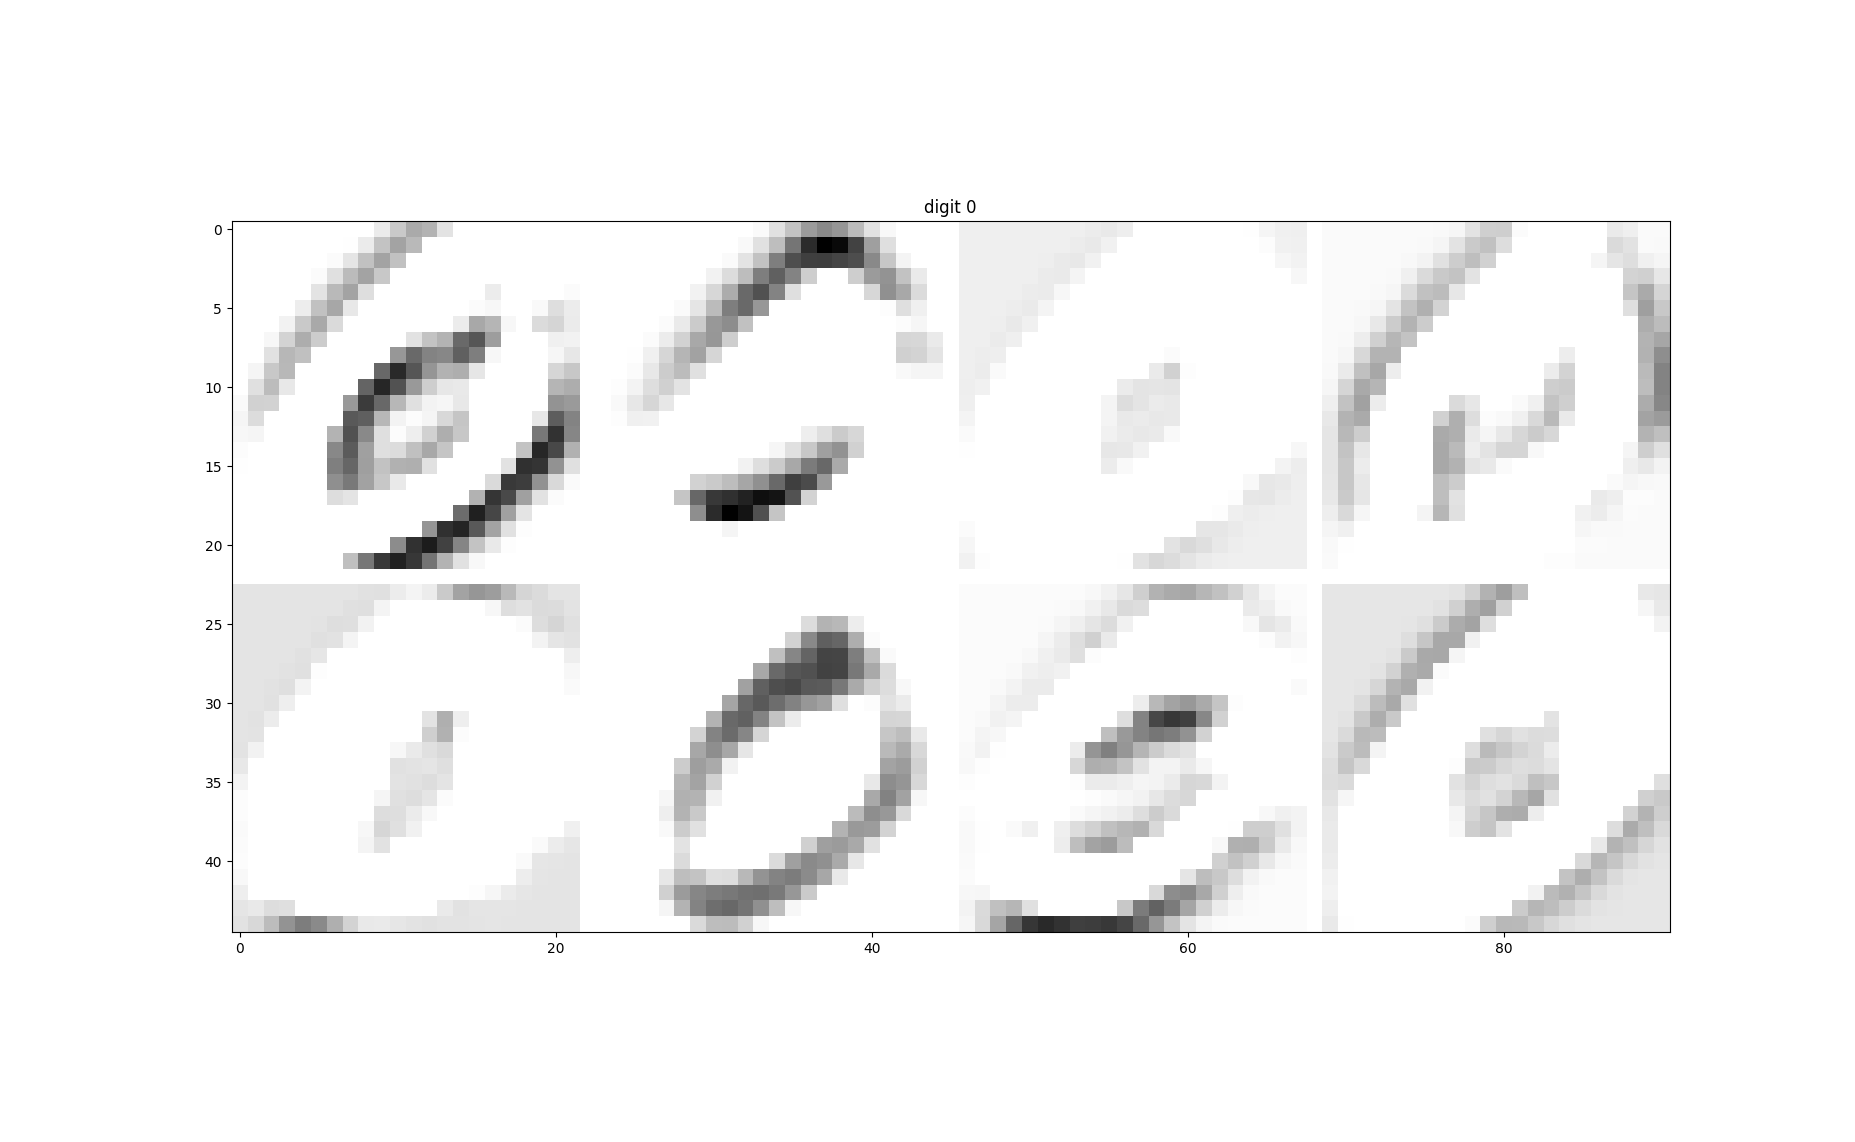
\includegraphics [scale=0.3]{digit0.png}
    \caption {feature map for digit 0}
\end{figure}

\begin{figure}[h]
    \centering
    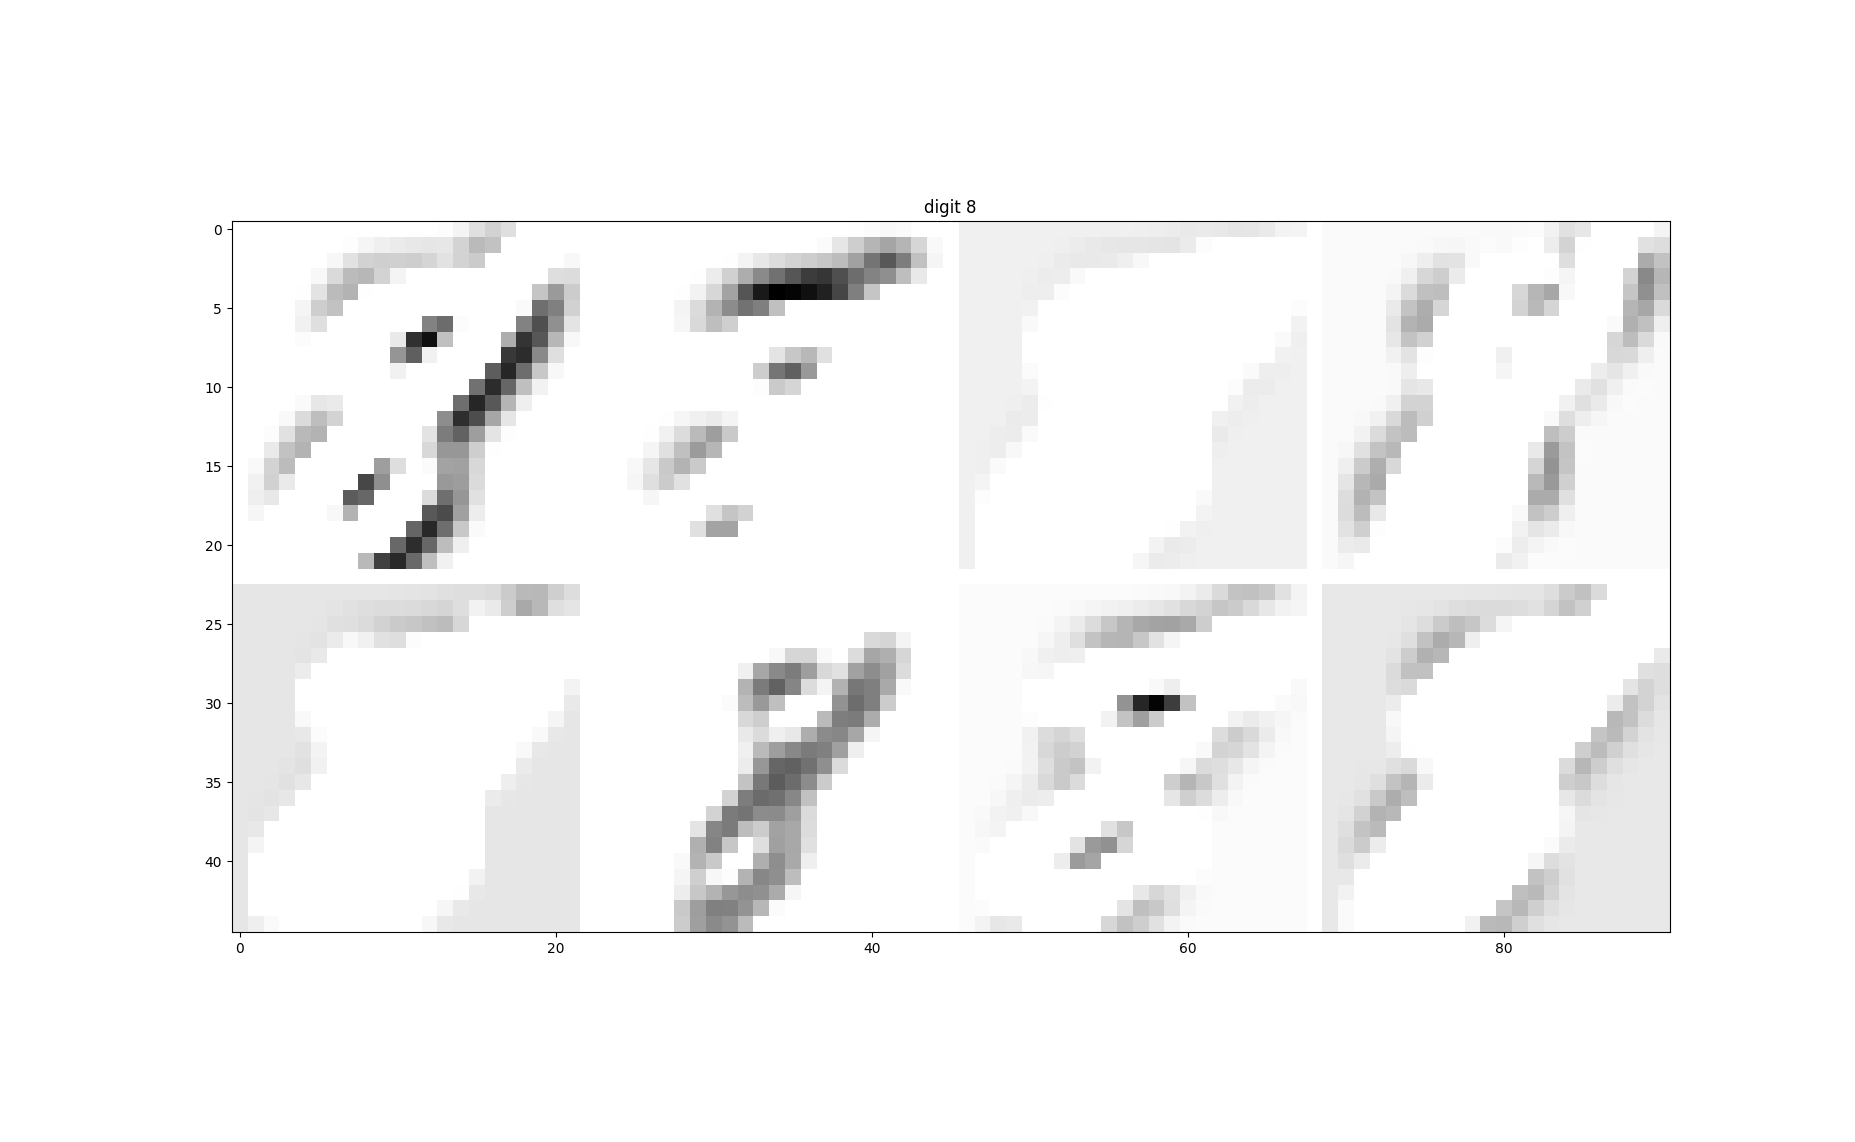
\includegraphics [scale=0.3]{digit8.png}
    \caption {feature map for digit 8}
\end{figure}
\clearpage

(3) The predictions do not change, they are still correctly labeled as
$1$.
\begin{figure}[h]
    \centering
    \begin{subfigure}[b]{0.32\linewidth}
    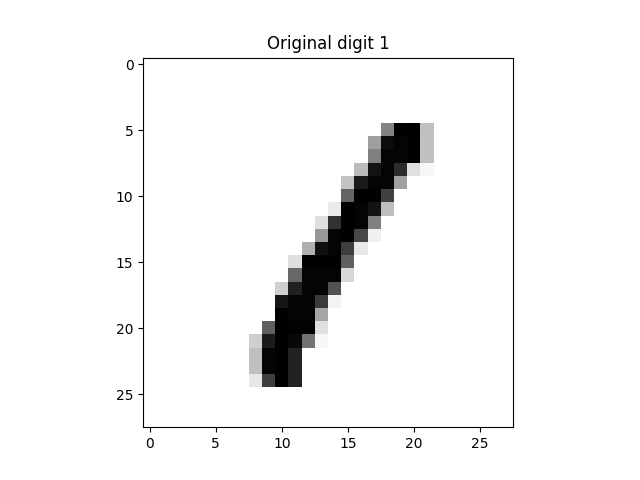
\includegraphics [width=\linewidth]{digit1_original.png}
    \caption {original}
    \end{subfigure}
    \begin{subfigure}[b]{0.32\linewidth}
    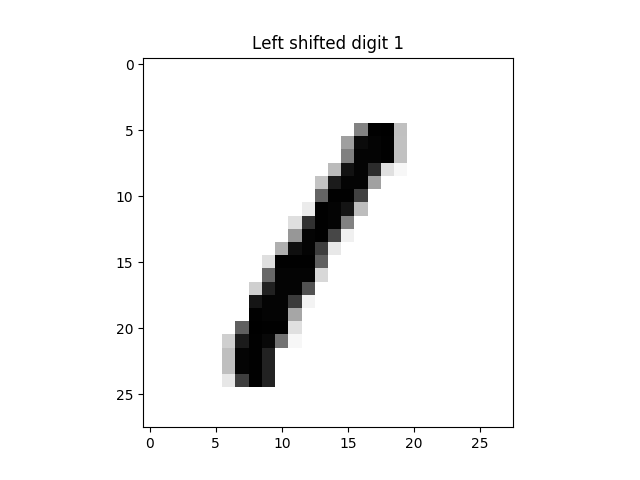
\includegraphics [width=\linewidth]{digit1_left.png}
    \caption {left shifted}
    \end{subfigure}
    \begin{subfigure}[b]{0.32\linewidth}
    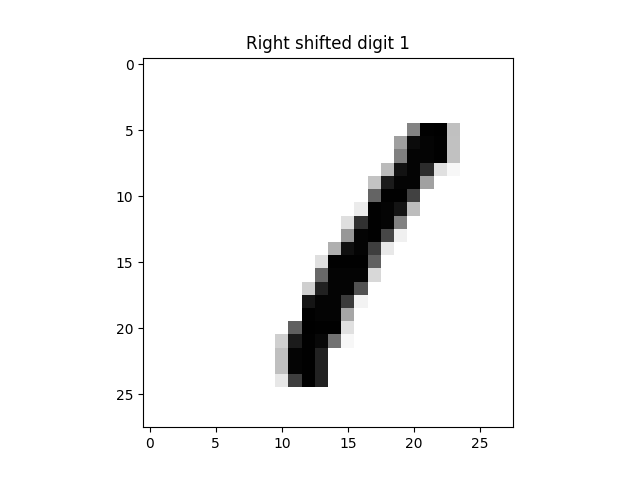
\includegraphics [width=\linewidth]{digit1_right.png}
    \caption {right shifted}
    \end{subfigure}
    \caption {digit 1}
\end{figure}
\clearpage

\section {Problem 2}
(1)
\begin{figure}[h]
    \centering
    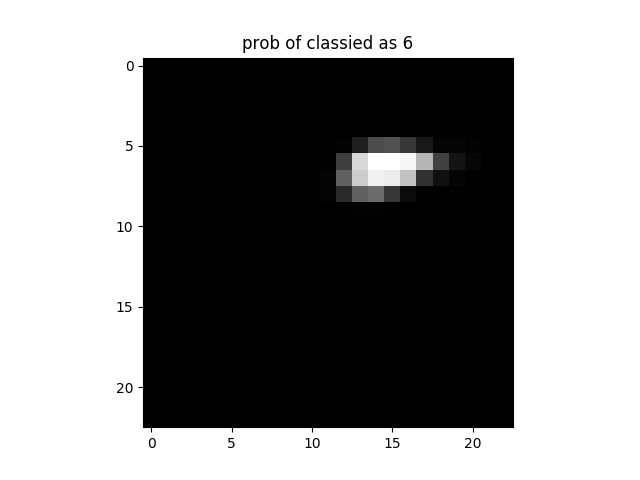
\includegraphics [scale=0.35]{digit6_prob_as_6.png}
    \caption {probability as 6}
\end{figure}

\begin{figure}[h]
    \centering
    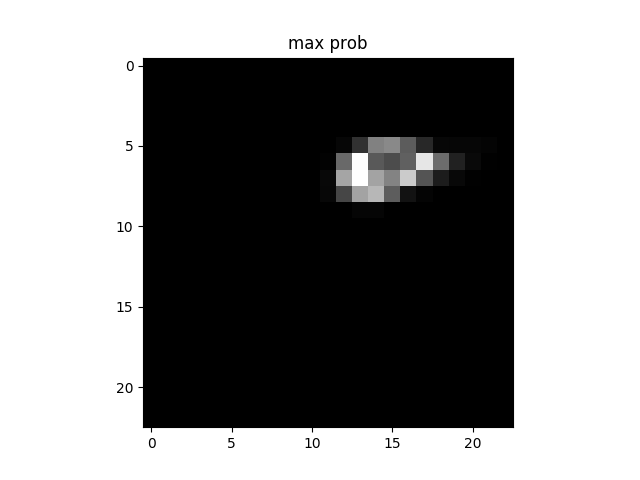
\includegraphics [scale=0.35]{digit6_max_prob.png}
    \caption {maximum probability}
\end{figure}

\begin{figure}[h]
    \centering
    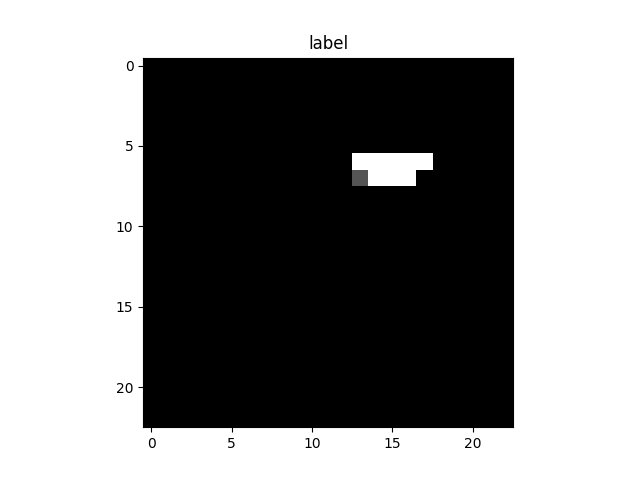
\includegraphics [scale=0.35]{digit6_label.png}
    \caption {label}
\end{figure}
\clearpage
(2) By analyse the hot spot, we can see most sensitive part is the
head of $6$, namely uper\--right corner of the figure. It's the most
important part for recogination.\\
(3) theoretically it can be done. Through the example in step 1, we
can see one black patch at the right location will lead to a
recogination of 4 or 0. It's presummed we can at least cut a black
patch from some digits and patch is at the hot spot, it might lead to
a $4$ or $0$. While I tried many times, and even increased the patch
size, It is still classied as $6$ somehow.

\section{Problem 3}
(1)\\
\begin{equation}
    \hat{y}^{(1)}=\begin{bmatrix} 0.94921601 \\ 0.05078399 \end{bmatrix}, \quad
    \hat{y}^{(2)}=\begin{bmatrix} 0.95221995 \\ 0.04778005 \end{bmatrix}, \quad
    \hat{y}^{(3)}=\begin{bmatrix} 0.94001124 \\ 0.05998876 \end{bmatrix}
\end{equation}
loss:  9.434827012614068\\
(2)
\begin{equation}
    L(b_1-\epsilon)= 9.434835467223774, \quad
    L(b_1+\epsilon)= 9.43481855635174
\end{equation}

\begin{equation}
    \frac{dL}{db_1}\approx -0.08455436017129614
\end{equation}

\begin{equation}
    L(b_2-\epsilon)= 9.434775274858213 , \quad
    L(b_2+\epsilon)= 9.434878741709078
\end{equation}

\begin{equation}
    \frac{dL}{db_2}\approx 0.5173342543240977
\end{equation}

(3) The backpropogation is calculated as:\\
\begin{equation}
    \frac{dl}{d\hat y}=
    \begin{bmatrix} \frac{dl}{d\hat y_1} \\ \frac{dl}{d\hat y_2} \end{bmatrix}=
    \begin{bmatrix} 2\hat y_1-1 \\ -\frac{1}{\hat y_2} \end{bmatrix}
\end{equation}

\begin{equation}
    \frac{dl}{do}=(\frac{d\hat y}{do})^T.dot(\frac{dl}{d\hat y})
\end{equation}

in which
\begin{equation}
\frac{d \hat y}{do}=\hat y _1 \hat y _2\begin{bmatrix} 1 \quad -1\\
                                                 -1 \quad  1 \end{bmatrix}\\
\end{equation}

\begin{equation}
    \frac{dl}{dh}=(\frac{do}{dh})^T.dot(\frac{dl}{do})=V^T.dot(\frac{dl}{do})
\end{equation}

\begin{equation}
    \frac{dl}{da}=\frac{dh}{da}*\frac{dl}{dh}=(1-h^2)*\frac{dl}{dh}
\end{equation}

\begin{equation}
    \frac{dl}{db}=(\frac{da}{db})^T.dot(\frac{dl}{da})
\end{equation}

in which\\
\begin{equation}
    \frac{da}{db}=\begin{bmatrix} 1 \quad 0 \\ 0 \quad 1
    \end{bmatrix}+W.dot(\frac{dh^{t-1}}{db})
\end{equation}

in which\\
\begin{equation}
    \frac{dh^{t-1}}{db}=((\frac{da^{t-1}}{db})^T*\frac{dh^{t-1}}{da^{t-1}})^T
\end{equation}

All these notations follow the Python standards, in which $*$ stands
    for element\--wise multiplication.
Results:\\
For $t=0$:\\
$\frac{dl}{dy}=\begin{bmatrix} 0.89843201 \\ -19.691243652 \end{bmatrix}$\\
$\frac{dy}{do}=\begin{bmatrix} 0.04820498 \quad -0.04820498\\
                              -0.04820498 \quad  0.04820498 \end{bmatrix}$\\
$\frac{dl}{do}=\begin{bmatrix} 0.9925249 \\ -0.9925249\end{bmatrix}$\\
$\frac{do}{dh}=\begin{bmatrix} -2 \quad 1\\
                               -1 \quad 0 \end{bmatrix}$\\
$\frac{dl}{dh}=\begin{bmatrix} -0.9925249 \\ 0.9925249\end{bmatrix}$\\
$\frac{dl}{da}=\begin{bmatrix} -0.0701227 \\ 0.0701227\end{bmatrix}$\\
$\frac{da}{db}=\begin{bmatrix} 1 \quad 0\\
                               0 \quad 1 \end{bmatrix}$\\
$\frac{dl}{db}=\begin{bmatrix} -0.0701227 \\ 0.0701227\end{bmatrix}$\\

For $t=1$:\\
$\frac{dl}{dy}=\begin{bmatrix} 0.9044399 \\ -20.9292368\end{bmatrix}$\\
$\frac{dy}{do}=\begin{bmatrix} 0.04549712 \quad -0.04549712 \\
                              -0.04549712 \quad  0.04549712  \end{bmatrix}$\\
$\frac{dl}{do}=\begin{bmatrix} 0.99336936 \\ -0.99336936\end{bmatrix}$\\
$\frac{do}{dh}=\begin{bmatrix} -2 \quad 1\\
                               -1 \quad 0 \end{bmatrix}$\\
$\frac{dl}{dh}=\begin{bmatrix} -0.99336936 \\ 0.99336936\end{bmatrix}$\\
$\frac{dh}{da}=\begin{bmatrix} 0.00420315 \\ 0.01138416\end{bmatrix}$\\
$\frac{dl}{da}=\begin{bmatrix} -0.00417528 \\ 0.01130867\end{bmatrix}$\\
$\frac{dh}{db}=\begin{bmatrix} 0.07065082 \quad 0. \\
                               0. \quad 0.07065082\end{bmatrix}$\\
$\frac{da}{db}=\begin{bmatrix} 1.07065082 \quad -0.07065082\\
                               0. \quad          1.14130165 \end{bmatrix}$\\
$\frac{dl}{db}=\begin{bmatrix} -0.00447027 \\  0.0132016\end{bmatrix}$\\

For $t=2$:\\
$\frac{dl}{dy}=\begin{bmatrix} 0.88002248 \\ -16.66978991\end{bmatrix}$\\
$\frac{dy}{do}=\begin{bmatrix}  0.05639011 \quad -0.05639011 \\
                               -0.05639011 \quad 0.05639011  \end{bmatrix}$\\
$\frac{dl}{do}=\begin{bmatrix} 0.9896358 \\ -0.9896358\end{bmatrix}$\\
$\frac{do}{dh}=\begin{bmatrix} -2 \quad 1\\
                               -1 \quad 0 \end{bmatrix}$\\
$\frac{dl}{dh}=\begin{bmatrix} -0.9896358 \\ 0.9896358\end{bmatrix}$\\
$\frac{dh}{da}=\begin{bmatrix} 0.01002062 \\ 0.42731798\end{bmatrix}$\\
$\frac{dl}{da}=\begin{bmatrix} -0.00991676 \\ 0.42288917\end{bmatrix}$\\
$\frac{dh}{db}=\begin{bmatrix} 0.00450011\quad -0.00029696 \\
                               0.\quad          0.01299276\end{bmatrix}$\\
$\frac{da}{db}=\begin{bmatrix} 1.00450011 \quad -0.01328971\\
                               0.         \quad 1.02598552 \end{bmatrix}$\\
$\frac{dl}{db}=\begin{bmatrix} -0.00996139 \\  0.43400995\end{bmatrix}$\\
    Add these 3 $\frac{dl}{db}$, we get
\begin{equation}
    \frac{dl}{db}=\begin{bmatrix} -0.08455436 \\0.51733425\end{bmatrix}
\end{equation}
    which is almost
    the same with the central difference results.\\
(4) new $b$:
\begin{equation}
     b=\begin{bmatrix} -1.00084554 \\ 1.00517334\end{bmatrix}
\end{equation}

(5) new loss with new $b$ 9.437563229688841

\section{Problem 4}
(1) The most difficult part should be $W$ and $U$, if we unfold the graph, we
can see $W$ connects the hidden states for different time steps, we
need to do a backpropogation for $W$ and $U$ for all preceding time step.
Long\--time dependence is very difficult to train. \\
(2) echo state network fixes $W$ and $U$. Only $V$ is learned.\\
(3) By adding forget gates and input gates, vanish gradient introduced
by long\--time dependence can be aleviated.

\end{document}
